\documentclass[a4paper, 11pt]{article}

%%% Packages
\usepackage[margin=50pt, vmargin={50pt, 10pt},includefoot]{geometry}
\usepackage{palatino}
\usepackage{graphicx}
\DeclareGraphicsExtensions{.pdf,.png,.jpg}
%%% Listing package
\usepackage{listings}
\usepackage{color}
\usepackage{url}
\usepackage{hyperref}

\hypersetup{
  colorlinks = false,
  pdfborder={0 0 0}
}

\definecolor{dkgreen}{rgb}{0,0.6,0}
\definecolor{gray}{rgb}{0.5,0.5,0.5}
\definecolor{mauve}{rgb}{0.58,0,0.82}
\definecolor{red}{rgb}{0.8,0,0}

\lstset{ 
  language=C++,                % the language of the code
  basicstyle=\footnotesize,           % the size of the fonts that are used for the code
  numbers=left,                   % where to put the line-numbers
  numberstyle=\tiny\color{gray},  % the style that is used for the line-numbers
  stepnumber=0,                   % the step between two line-numbers. If it's 1, each line 
  numbersep=5pt,                  % how far the line-numbers are from the code
  backgroundcolor=\color{white},      % choose the background color. You must add \usepackage{color}
  showspaces=false,               % show spaces adding particular underscores
  showstringspaces=false,         % underline spaces within strings
  showtabs=false,                 % show tabs within strings adding particular underscores
  frame=single,                   % adds a frame around the code
  rulecolor=\color{black},        % if not set, the frame-color 
  captionpos=b,                   % sets the caption-position to bottom
  breaklines=true,                % sets automatic line breaking
  breakatwhitespace=false,        %sets if automatic breaks should only happen at whitespace
  title=\lstname,                   % show the filename of files included with \lstinputlisting;
  keywordstyle=\color{blue},         % keyword style
  keywordstyle=[2]\color{dkgreen},
  commentstyle=\color{red},       %comment style
  keywords=[2]{DataType, ClosedType, FringeType, ClosedTypeIterator, CompareByState, CompareByCost},
  stringstyle=\color{mauve},         %string literal style
  escapeinside={\%*}{*)},            % if you want to add LaTeX within your code
  emph={string, Puzzle, Board, multiset},  % emphasized characters
  emphstyle={\color{dkgreen}}
}

%%% End listing

\begin{document}
\title{Artificial Intelligence Report 7th Week-23rd Problem}
\author{Le Trung Kien\\ 
  03-120291, 3rd Year \\
  Department of Mechano-Informatics \\ 
  The University of Tokyo
}
\maketitle

\section*{Note}
\begin{itemize}
\item Required libraries: Eigen, OpenCV
\item The executable files should work fine, but compiling the source code is hard due to libraries' configuration.
\end{itemize}

\newpage
\section{Backpropagation Neural Network}
The prototype for Backpropagation Neural Network (BnnnnPNN) is shown in Listing 1.
\begin{lstlisting}[caption={Backpropagation Neural Network Class (bpnn.hpp)}]
class BPNN{
private:
    vector<MatrixXd> weight;
    vector<MatrixXd> weightGrad;
    vector<MatrixXd> prevWeightGrad;
    vector<MatrixXd> delta;
    vector<MatrixXd> output;
    vector<MatrixXd> buffer;
    vector<int> layerSize;
    void Update(double learningRate, double momentum, int iteration, int maxIteration);
    bool CheckConvergence(double prev, double current, double min, double threshold);
public:
    enum WeightInitType {RANDOM, ZEROS};
    BPNN();
    BPNN(const vector<int> &layerSize);
    BPNN(int inputLayerSize, int hiddenLayerSize, int outputLayerSize);
    void Initialize(const vector<int>& layerSize);
    void Compute(const MatrixXd &in, MatrixXd& out);
    void Compute(const MatrixXd &in);
    void ComputeAll(const MatrixXd &in, MatrixXd& out);
    double Run(const MatrixXd &in, const MatrixXd &out);
    double RunEpoch(const MatrixXd &trainInput, const MatrixXd &trainOutput, double lambda);
    BPNN Train(const MatrixXd &trainInput, const MatrixXd &trainOuput, 
	       double learningRate, double lambda, double momentum, 
               int maxIteration, double threshold);
    void Predict(const MatrixXd &in, MatrixXd &out, MatrixXd &outputLabel);
    void Save(const string& filename);
    void Load(const string& filename);
    void SetWeight(const vector<MatrixXd> &weight);
    void SetWeight(WeightInitType type = RANDOM);
    vector<MatrixXd> Weight() const;
    MatrixXd Output() const;
    vector<int> LayerSize() const;
    int InputLayerSize() const ;
    int OutputLayerSize() const ;
    int LayerNum() const ;
};
\end{lstlisting}
I am not going to talk much about BPNN's implementation, since it is very straightforward. Details about BPNN's theory can be seen in [\ref{itm:PRML}]. The most important method and its parameters of BPNN's class:
\begin{lstlisting}
BPNN Train(const MatrixXd &trainInput, const MatrixXd &trainOuput, 
           double learningRate, double lambda, double momentum, 
           int maxIteration, double threshold);
\end{lstlisting}
\begin{itemize}
\item \textbf{trainInput} input for training
\item \textbf{trainOuput} desired output for training
\item \textbf{learningRate} decides convergence's speed
\item \textbf{lambda} regularized parameter
\item \textbf{momentum} increases convergence's speed
\item \textbf{maxIteration} biggest number of iterations
\item \textbf{threshold} threshold to decide when error function converges
\end{itemize}
This method \textbf{returns} a trained BPNN which is ready for pattern's recognition.

\newpage
\section{Digit Recognition Application}
\subsection{Data preparation}
All the training and testing data which consists of 900 grayscale images are pulled from MNIST's database.
\begin{center}\url{http://yann.lecun.com/exdb/mnist/}\end{center}
All images have size of 20x20. Pixcell's value is scaled from [0,255] range to [0,1] range. They are put into a single xml file along side with a xml file containing respective labels.
\begin{figure}[ht]
  \centering
  
\includegraphics[scale=5]{img0014}
  \caption{An image of 9}
  \label{fig:9}
\end{figure}
Noise is not directly generated from data but labels. In this report, noise should be solely thought as mislabelled images.
\subsection{Experiments}
In my experiements, data are divided into the following three sets.
\begin{enumerate}
\item \textbf{Training Set} is used for BPNN's training. Its size varies from 20 to 700.
\item \textbf{Cross Validation Set} is used to check for overfitting and optimal parameters' selection. It includes 100 images.
\item \textbf{Test Set} is used to check trained network's precision. It includes 100 images.
\end{enumerate}
Firstly, I exam how training set's size affects BPNN's performance. In this experiment, hidden layer has 10 neurons, and regularized parameter is 0. As shown in Figure 2 and 3, as the size of the training set increases, the training error increases while the cross validation error decreases. Figure 2 shows that relationship when no noise involves, while Figure 3 shows it with 25\% of noise. In both cases, the precision is going up as the training set's size increases, though in different trajectory.

\begin{figure}[t]
  \centering
  %%% hiddne = 10, lambda = 0, noise = 25%
  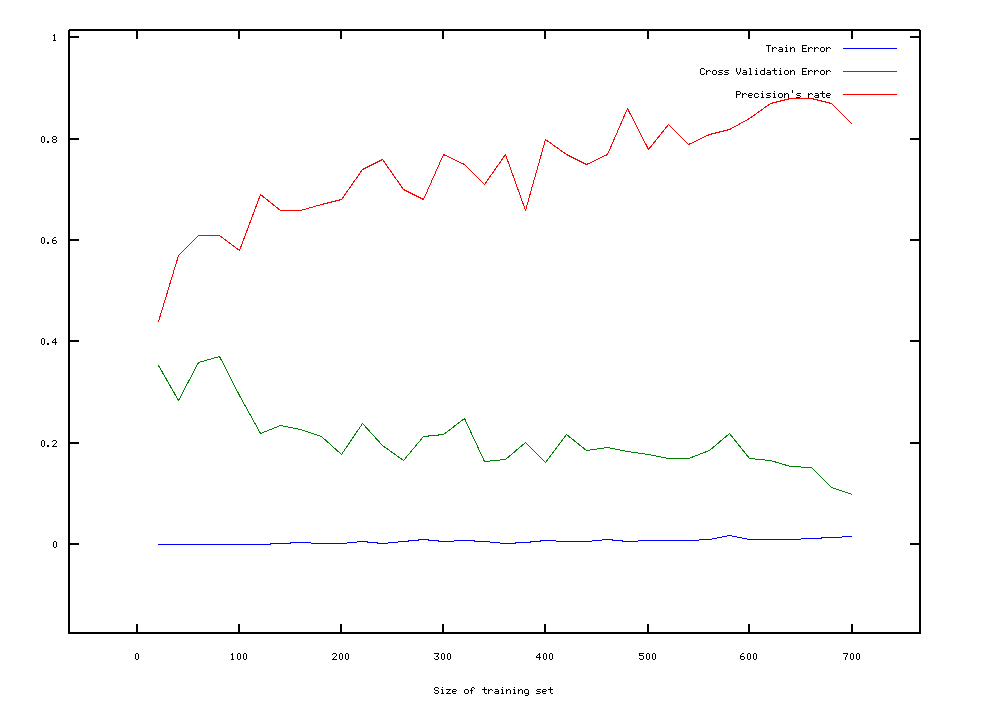
\includegraphics[scale=0.45]{1}
  \caption{Training error and cross validation error as functions of training set's size without noise.}
  \label{fig:m1}
  %%% hiddne = 10, lambda = 0, noise = 25%
  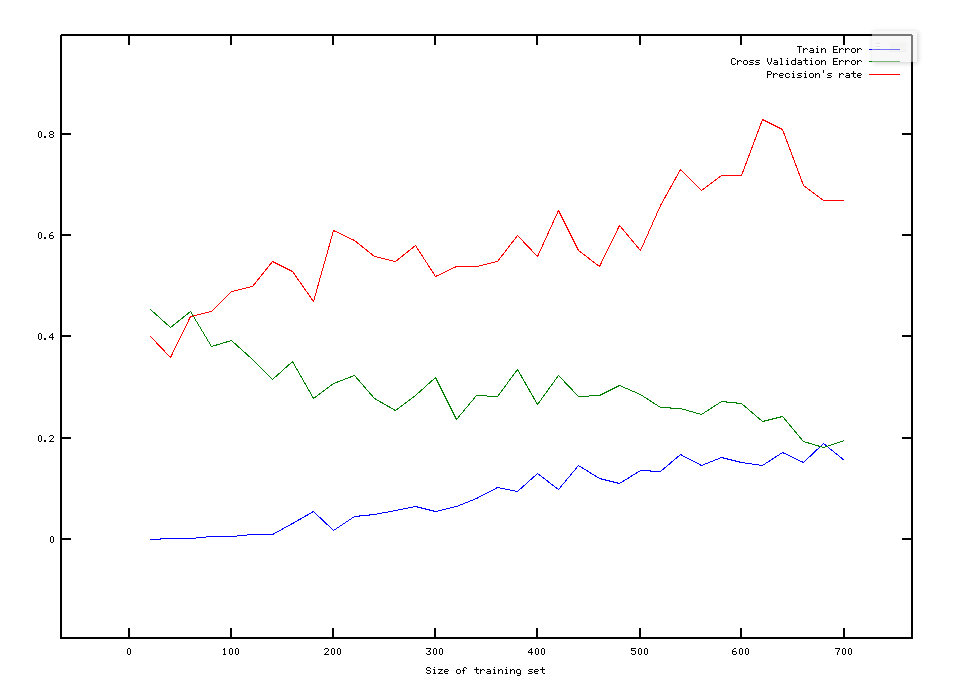
\includegraphics[scale=0.45]{2}
  \caption{Training error and cross validation error as functions of training set's size with 25\% of noise.}
  \label{fig:m2}
\end{figure}

Secondly, we exam how BPNN's precision is reduced after adding noise to training set. Hidden layer size is 10, training set size is 300. According to Figure 4, the more noise the training set has, the larger the cross validation error is and the lower the precision is. \\
Finally, I want to figure 
\begin{figure}[t]
  \centering
  %%% hiddne = 10, lambda = 0, m = 300
  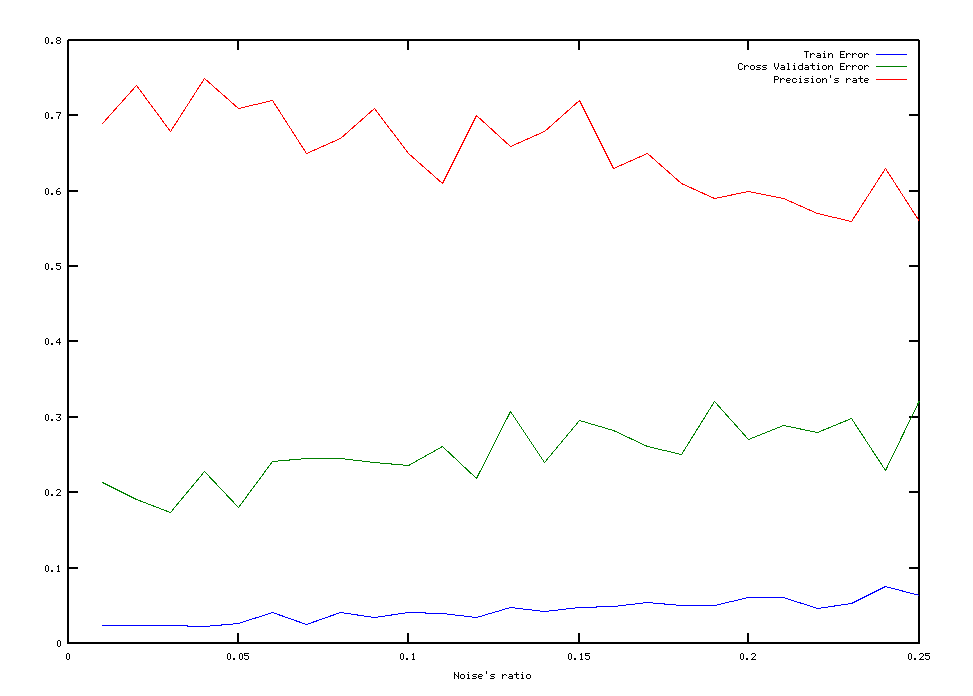
\includegraphics[scale=0.45]{3}
  \caption{Training, cross validation errors and precision's relationships with noise's ratio in training set.}
  \label{fig:m3}
\end{figure}

% \newpage
\begin{thebibliography}{9}
\bibitem{PRML}
  \label{itm:PRML}
  Christopher M. Bishop
  \emph{Pattern Recognition and Machine Learning},
  Springer
  1st Edition,
  2006

\end{thebibliography}

\end{document}